\documentclass[12pt]{article}
\usepackage[top=1in, bottom=1in, left=.75in, right=.75in]{geometry}
\usepackage{amsmath}
\usepackage{fancyhdr}
\usepackage{graphicx}
\usepackage{txfonts}
\usepackage{multicol,coordsys}
\usepackage[scaled=0.86]{helvet}
\renewcommand{\emph}[1]{\textsf{\textbf{#1}}}
\usepackage{anyfontsize}
\usepackage[shortlabels]{enumitem}
% \usepackage{times}
% \usepackage[lf]{MinionPro}
\usepackage{tikz,pgfplots,mathrsfs}
%\def\degC{{}^\circ{\rm C}}
\def\ra{\rightarrow}
\usetikzlibrary{calc, backgrounds}
\pgfplotsset{compat = newest}
\newcommand{\blank}[1]{\rule{#1}{0.75pt}}

\pgfplotsset{my style/.append style={axis x line=middle, axis y line=
middle, xlabel={$x$}, ylabel={$y$},axis equal}}

%yticklabels={,,} , xticklabels={,,}

% \setmainfont{Times}
% \def\sansfont{Lucida Grande Bold}
\parindent 0pt
\parskip 4pt
\pagestyle{fancy}
\fancyfoot[C]{\emph{\thepage}}
\fancyhead[L]{\ifnum \value{page} > 1\relax\emph{Math 252: Midterm Exam 1}\fi}
\fancyhead[R]{\ifnum \value{page} > 1\relax\emph{Spring 2024}\fi}
\headheight 15pt
\renewcommand{\headrulewidth}{0pt}
\renewcommand{\footrulewidth}{0pt}
\let\ds\displaystyle
\def\continued{{\emph {Continued....}}}
\def\continuing{{\emph {Problem \arabic{probcount} continued....}}\par\vskip 4pt}

\newcommand{\prob}[1]{\bigskip\noindent\textbf{#1.} }
\newcommand{\pts}[1]{(\emph{#1 pts})}

\newcommand{\probpts}[2]{\prob{#1} \pts{#2} \quad}
\newcommand{\ppartpts}[2]{\textbf{(#1)} \pts{#2} \quad}
\newcommand{\epartpts}[2]{\medskip\noindent \textbf{(#1)} \pts{#2} \quad}

%\newcounter{probcount}
%\newcounter{subprobcount}
%\newcommand{\thesubproblem}{\emph{\alph{subprobcount}.}}
%\def\problem#1{\setcounter{subprobcount}{0}%
%\addtocounter{probcount}{1}{\emph{\arabic{probcount}.\hskip 1em(#1)}}\par}
%\def\subproblem#1{\par\hangindent=1em\hangafter=0{%
%\addtocounter{subprobcount}{1}\thesubproblem\emph{#1}\hskip 1em}}
%\def\probskip{\vskip 10pt}
%\def\medprobskip{\vskip 2in}
%\def\subprobskip{\vskip 45pt}
%\def\bigprobskip{\vskip 4in}

\begin{document}
{\emph{\fontsize{26}{28}\selectfont Math F252 (Bueler)\hfill
{\fontsize{32}{36}\selectfont Midterm I}
\hfill Spring 2024}}
\vskip 2cm
\strut\vtop{\halign{\emph#\hskip 0.5em\hfil&#\hbox to 2in{\hrulefill}\cr
\emph{\fontsize{18}{22}\selectfont Name:}&\cr
\noalign{\vskip 10pt}}}
%%\emph{\fontsize{18}{22}\selectfont Student Id:}&\cr
%%\noalign{\vskip 10pt}
%%\emph{\fontsize{18}{22}\selectfont Calculator Model:}&\cr
%}}
%\hfill
%\vtop{\halign{\emph{\fontsize{18}{22}\selectfont #}\hfil& \emph{\fontsize{18}{22}\selectfont\hskip 0.5ex $\square$ #}\hfil\cr
%Section: & 001 (Jill Faudree)\cr
%\noalign{\vskip 4pt}
%         & 002 (James Gossell)\cr
%\noalign{\vskip 4pt}
%         & 005 (James Gossell)\cr}}

\vfill
{\fontsize{18}{22}\selectfont\emph{Rules:}}

You have {90 minutes} to complete this midterm.  

Partial credit will be awarded, but you must show your work.

%You may have a single handwritten $3 \times 5$ notecard.
%Calculators are not allowed. 
Notes, books, calculators, and internet access are not allowed. 

%Place a box around your  \fbox{FINAL ANSWER} to each question where appropriate.
Circle or box your \fbox{FINAL ANSWER} to each question where appropriate.

%If you need extra space, you can use the back sides of the pages.
%Please make it obvious  when you have done so.

Turn off anything that might go beep during the exam.

Good luck!
\vfill
\def\emptybox{\hbox to 2em{\vrule height 16pt depth 8pt width 0pt\hfil}}
\def\tline{\noalign{\hrule}}
\centerline{\vbox{\offinterlineskip
{
\bf\sf\fontsize{18pt}{22pt}\selectfont
\hrule
\halign{
\vrule#&\strut\quad\hfil#\hfil\quad&\vrule#&\quad\hfil#\hfil\quad
&\vrule#&\quad\hfil#\hfil\quad&\vrule#\cr
height 3pt&\omit&&\omit&&\omit&\cr
&Problem&&Possible&&Score&\cr\tline
height 3pt&\omit&&\omit&&\omit&\cr
&1&&10&&\emptybox&\cr\tline
&2&&6&&\emptybox&\cr\tline
&3&&16&&\emptybox&\cr\tline
&4&&10&&\emptybox&\cr\tline
&5&&10&&\emptybox&\cr\tline
&6&&14&&\emptybox&\cr\tline
&7&&24&&\emptybox&\cr\tline
&8&&10&&\emptybox&\cr\tline
&Extra Credit&&5&&\emptybox&\cr\tline
&Total&&100&&\emptybox&\cr
}\hrule}}}

\newpage
\prob{1}\ppartpts{a}{3} Use the graphs below to shade the region bounded by $y=e^{x/2},$ $y=e^{x-1}$ and $x=0.$\\

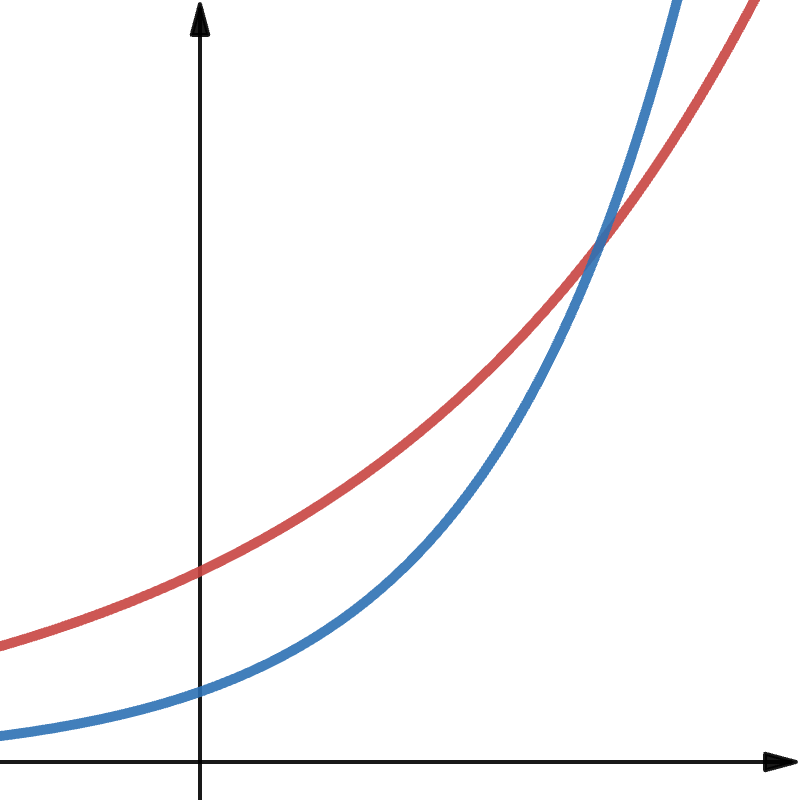
\includegraphics[scale=0.2]{m1p1.png}

\epartpts{b}{7} Determine the area of this region using an appropriate integral. \\

%\textcolor{red}{This is just like a homework problem.}
\vfill
\probpts{2}{6} Set up but do not evaluate an integral computing the arc length of the curve $y=\tan(x^2)$ between $x=-\pi/4$ to $x=\pi/4$.\\
\vspace{1.5in}

\newpage
\prob{3}\ppartpts{a}{2} Sketch the region bounded by the curves $y=x^2$ and $y=2x.$
\vspace{2in}

\epartpts{b}{6} Use an integral to compute the volume of the solid found by rotating the region in part $\textbf{a.}$ around the $x$-axis.
\vfill
\epartpts{c}{4} Use the \emph{shell method} to set up an integral to calculate the volume of the solid obtained by rotating the region in part $\textbf{a.}$ around the $y$-axis. You do not need to evaluate the integral.

\vspace{1.3in}

\epartpts{d}{4} Use the \emph{slicing method} (disks/washers) to set up an integral to calculate the volume of the solid obtained by rotating the region in part $\textbf{a.}$ around the $y$-axis. You do not need to evaluate the integral.

\vspace{1in}

\newpage

\probpts{4}{10} A 3-meter long whip antenna has linear density $\rho(x)=5-\frac{1}{x+1}$ grams per centimeter (starting at $x=0$). Determine the mass of the antenna. Include units.

\vfill

\probpts{5}{10} A 1-meter spring requires 20 J to compress the spring to a length of $0.9$ meters. How much work would it take to compress the spring from 1 meter to $0.8$ meters?
\vfill 
\newpage
\prob{6} Evaluate the definite integrals. Simplify your answers\\
\epartpts{a}{7} $\ds \int_0^{\pi/4} \tan \theta \: d\theta$
\vfill
\epartpts{b}{7} $\ds \int_0^2 xe^{3x}\: dx $
\vfill


\newpage
\prob{7} Evaluate the indefinite integrals.\\
\epartpts{a}{6} $\ds \int \sin^3(4x)\cos^2(4x)\: dx $
\vfill
\epartpts{b}{6} $\ds \int \sec^4(x)\: dx $
\vfill

\newpage
\epartpts{c}{6} $\ds \int \arcsin(x) \: dx$
\vfill
\epartpts{d}{6} $\ds \int \frac{2}{(2x+1)(2x-3)} \: dx$
\vfill
\newpage
\probpts{8}{10} Use the method of Trigonometric Substitution to evaluate the integral $\ds \int \frac{dx}{(4+x^2)^2}.$ Your final answer must be simplified and written in terms of $x.$
\newpage
\prob{Extra Credit} A particle moving along a straight line has a velocity of $v(t)=te^{-t}$ after $t$ seconds where $v$ is measured in meters per second.

 \epartpts{a}{2} How far does the particle travel from time $t=0$ seconds to time $t=T$ seconds?
\vfill
\epartpts{b}{3} Use your answer from part \textbf{a.} to determine how far the particle travels in the long-term, as $T \to \infty.$
\vfill

\hrulefill

You may find the following \textbf{trigonometric formulas} useful.  Other formulas, not listed here, should be in your memory, or you can derive them from the ones here.
\begin{align*}
\sin(\alpha \pm \beta) &= \sin \alpha \cos \beta \pm \cos \alpha \sin \beta \qquad &
    \sin(ax) \sin(bx) &= \frac{1}{2} \cos((a-b)x) - \frac{1}{2} \cos((a+b)x) \\
\cos(\alpha \pm \beta) &= \cos \alpha \cos \beta \mp \sin \alpha \sin \beta \qquad &
    \sin(ax) \cos(bx) &= \frac{1}{2} \sin((a-b)x) + \frac{1}{2} \sin((a+b)x) \\
 && \cos(ax) \cos(bx) &= \frac{1}{2} \cos((a-b)x) + \frac{1}{2} \cos((a+b)x)
\end{align*}
\end{document}